\documentclass{beamer}
\usepackage[utf8]{inputenc}
\usepackage[french]{babel}
\usepackage{graphics}
\usepackage{multirow}
\usepackage{colortbl}
\usepackage{CJKutf8}
\usepackage{colortbl}
\usepackage{changepage}

%\usepackage[screen,nopanel]{pdfscreen}
%\usepackage{url}

\usetheme{metropolis}

\definecolor{LightButter}{rgb}{0.98,0.91,0.31}
\definecolor{LightOrange}{rgb}{0.98,0.68,0.24}
\definecolor{LightChocolate}{rgb}{0.91,0.72,0.43}
\definecolor{LightChameleon}{rgb}{0.54,0.88,0.20}
\definecolor{LightSkyBlue}{rgb}{0.45,0.62,0.81}
\definecolor{LightPlum}{rgb}{0.68,0.50,0.66}
\definecolor{LightScarletRed}{rgb}{0.93,0.16,0.16}



\title{Mini-projet agile N3 2018}
\author{
  %\includegraphics[width=3cm]{logo_azae.png}
}
  
\date{}

\logo{
  \raisebox{-0.5\height}{\includegraphics[width=1cm]{cc_by_sa} }
}


\begin{document}

\frame{\titlepage}

\setbeamertemplate{frame footer}{https://gitlab.com/tclavier/intro-projet-agile-iut}

\begin{frame}{C'est quoi ?}
 
  {\Large \alert{Être agile} et pas faire de l'Agile.}

  \vspace{6mm}
  C'est avant tout un état d'esprit partagé par l'ensemble des participants à un projet.
\end{frame}

\begin{frame}{Être agile}
  "Les firmes qui survivent dans le long terme ne sont pas celles qui sont les plus fortes ou les plus intelligentes, mais celles qui s'adaptent le mieux aux changements d'environnement"

  \flushright{Hiroshi Okuda, Toyota}

\end{frame}

\begin{frame}{Le manifeste agile}
  \large
  \alert{Individuals and interactions} over processes and tools\newline
  \alert{Working software} over comprehensive documentation\newline
  \alert{Customer collaboration} over contract negotiation\newline
  \alert{Responding to change} over following a plan
\end{frame}

\begin{frame}{Valeurs et principes}
  \Large Des cycles courts, un produit en production à chaque fin de cycle et des producteurs de valeurs qui s'améliorent continuellement.
\end{frame}

\begin{frame}{Scrum : déroulé}
  \center
  \includegraphics[width=10cm]{includes/scrum1}
\end{frame}

\begin{frame}{Scrum : les rituels}
  \center
  \includegraphics[width=10cm]{includes/scrum2}
\end{frame}

\begin{frame}{Scrum : les rôles}
  \center
  \includegraphics[width=10cm]{includes/scrum3}
\end{frame}

\begin{frame}{Scrum : le mini-projet agile}
  \center
  \includegraphics[width=10cm]{includes/simulation}
\end{frame}

\begin{frame}{Le radiateur d'information}
  \begin{itemize}
    \item Donner les moyens aux acteurs d'être autonomes
    \item Faire rayonner l'information (donc pas de Trello ou Jira)

    \begin{itemize}
      \item Vision du projet, Proposition de valeur unique
      \item Date de livraison, avancement, etc.
      \item Planing des congés
      \item Actions d'améliorations
      \item Backlog
      \item Problèmes
      \item Etc.
    \end{itemize}
  \end{itemize}
\end{frame}

\begin{frame}{Exemple de radiateur}
  \center
  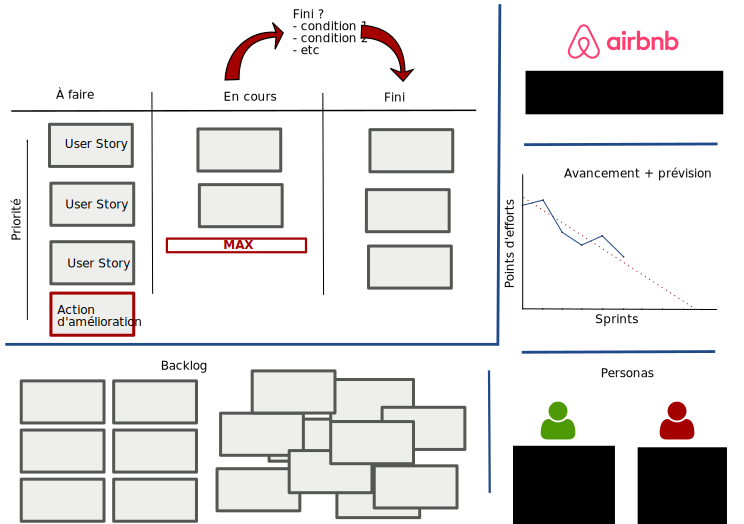
\includegraphics[width=10cm]{includes/radiateur}
\end{frame}

\begin{frame}{Kaizen 
    {\begin{CJK*}{UTF8}{mj} 改善 \end{CJK*}}
  }
  \center
  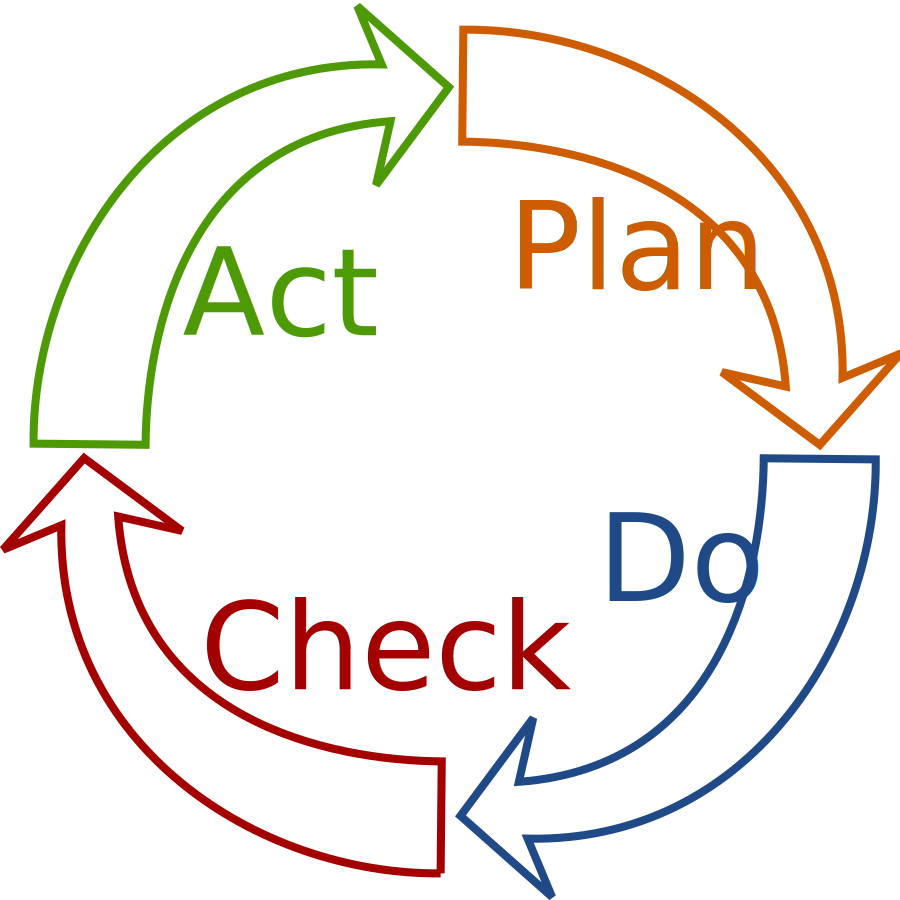
\includegraphics[width=6cm]{includes/pdca}
\end{frame}

\begin{frame}{Kaizen 
    {\begin{CJK*}{UTF8}{mj} 改善 \end{CJK*}}
  }
  
  \begin{itemize}
    \item \alert{Plan} : Identifier une action d'amélioration et un élément observable qui pourra permettre de déterminer si l'action a porté ses fruits ou pas.
    \item \alert{Do} : Faire l'action sur un temps donné, une itération par exemple.
    \item \alert{Check} : Prendre le temps de mesurer si l'action a apporté le changement souhaité.
    \item \alert{Act} : Décider, l'action est peut-être à répéter, une autre action peut en découler, etc.
  \end{itemize}

\end{frame}

\newcolumntype{g}{>{\columncolor[gray]{0.8}}c}

\begin{frame}{Planing de la semaine}{}
  {
    \center
    \begin{tabular}{l | g | g | g  }
      & \textbf{05/09} & \textbf{06/09} \\
      \hline
      08h00 - 10h00 & Amphi + TD & Sprint \\
      \hline
      10h00 - 12h00 & Sprint 0   & Sprint \\
      \hline
      13h30 - 15h30 & Sprint     & Sprint \\
      \hline
      15h30 - 16h30 & Code       & Démo pour les S1 \\
      \hline
      17h30 - 18h30 & Sprint     & Rétrospective \\
      \hline
    \end{tabular}
  }

\end{frame}

\begin{frame}{Un Sprint}
  \begin{itemize}
    \item 1h30 de production
    \item 30 minutes pour s'améliorer
    \begin{itemize}
      \item Démo
      \item Rétrospective
      \item Action d'amélioration
    \end{itemize}
  \end{itemize}
\end{frame}

\begin{frame}{Détail du Sprint 0}
  2h, 4 Objectifs :
  \begin{itemize}
    \item Partager la vision du produit
    \item Découper et estimer le backlog
    \item Initier la pile technique et montrer que l'on est capable de livrer de la valeur.
    \item Construire la proposition de valeur unique :
    \begin{itemize}
      \item Cible
      \item Problème
      \item Solution
    \end{itemize}
  \end{itemize}
\end{frame}

\begin{frame}{Démo pour les S1}
  Vous devez convaincre que le travail réalisé durant les 2 jours était extraordinaire et montrer aux premières années ce qu'ils seront capables de faire dans 1 an.
  \begin{itemize}
    \item Montrez nous le résultat
    \item Expliquez ce que vous avez appris
  \end{itemize}
\end{frame}

\begin{frame}{Contraintes}
  \begin{itemize}
    \item Du java
    \item Une IHM en mode texte
    \item Slack pour les communications
    \item À chaque fin de sprint
    \begin{itemize}
      \item Un répertoire sprint-X
      \item avec dedans un fichier README.md
      \item et une photo du radiateur d'information
    \end{itemize}
  \end{itemize}
\end{frame}

\begin{frame}[fragile]{README.md}
  \tiny
  \begin{verbatim}
# Rétrospective de sprint X

Nom du scrum master du sprint : 

## Ce que nous avons fait durant ce sprint
Donnez ici la liste des histoires utilisateurs que vous avez livrés durant ce sprint.

## Ce que nous allons faire durant le prochain sprint
Donnez ici la liste des histoires utilisateurs que vous vous engagez à terminer durant le prochain sprint.

## PDCA 
### Qu'avons nous testé durant ce sprint ? 

### Qu'avons nous observé ? 

### Quelle décision prenons nous suite à cette expérience ? 

### Qu'allons nous tester durant les 2 prochaines heures ? 

### À quoi verra-t-on que celà à fonctionné ?

# Mémo
N'oubliez pas d'ajouter une photo du radiateur d'information au moment de la rétrospective.
  \end{verbatim}
\end{frame}



\begin{frame}{Équipes}
\Tiny
\begin{tabular}{l l l l l l}
\textbf{Équipe 1} & \textbf{Équipe 2} & \textbf{Équipe 3} & \textbf{Équipe 4} & \textbf{Équipe 5} & \textbf{Équipe 6} \\
BREVIERE Lu.  & BLANQUART Si.  & FOUANT Ma.     & CASSORET Ma. & DANGLOT Cl.   & BADAOUI Na.  \\
DARROMAN Ba.  & BLONDIN Lu.    & LECLERCQ Ga.   & CLUSMAN Lu.  & FERNANDES Ni. & CONGIN Ga.   \\
DOGIMONT Lu.  & DA CRUZ Ka.    & LIETAR Th.     & MANS Lé.     & GUILLEMIN Ré. & FOURNIER Hu. \\
FINOT El.     & DESREUMAUX Al. & OUTTIER Sa.    & OUVRY Th.    & LANNOY Fr.    & LECOCQ Va.   \\
PRACA Co.     & POULAIN Ro.    & REBEILLEAU Pi. & RANSON Fl.   & ONQUIERT An.  & PEDRO Ni.    \\
\\
\textbf{Équipe 7} & \textbf{Équipe 8} & \textbf{Équipe 9} & \textbf{Équipe 10} & \textbf{Équipe 11} & \textbf{Équipe 12} \\
BENNACER Mo.   & BLERREAU Al.   & BAUDRY Ma.   & CHOMBART Ga.  & BASCOP Ar.     & DELGRANGE Pi.  \\
BLOCH Sa.      & COUSSEMENT Ni. & BOURDIER Cl. & CLARISSE Ax.  & COLPART Ma.    & DURIEZ Qu.     \\
DEJONGHE Gr.   & FIEVET Fl.     & POTIER Fl.   & COPIN St.     & DESPELCHIN Br. & HANSON An.     \\
DELIESSCHE Qu. & PANNIER Ba.    & PRUNIER Fl.  & TELLIER Be.   & MASSON Ti.     & SHIPMAN Th.    \\
FORESTIER Na.  & PAYEN Cl.      & THEBAUD Em.  & VANRYSSEL Ju. & SOW Yo.        & VERZELE Ar.    \\
\\
\textbf{Équipe 13} & \textbf{Équipe 14} & \textbf{Équipe 15} & \textbf{Équipe 16} & \textbf{Équipe 17} & \textbf{Équipe 18} \\
BAUVIN Ra.  & \cellcolor[gray]{0.8} RABBOUJ Bi.& FLORENTIN Be.   & BAZIN Je.      & DELBROUCQ Al.  & COFFIN Ne. \\
DUHAMEL Al. & DUBOIS Gu.          & GRENIER Pi.     & DEGAND Ma.     & LAHOUSSE Lu.   & DEFEVER Co.\\
GELDHOF Su. & LABADIE Ni.         & \cellcolor[gray]{0.8}SPILMONT Mi. & KARAOUZENE Na. & LANDSCHOOT To. & LECOCQ Ma. \\
LETORET Ji. & MEERSSEMAN Lé.      & MARCANT Ai.     & MONCHEAUX Ba.  & PLAISANT Fl.   & MILHE Th.  \\
POTEAU Al.  & PEREIRA Ni.         & PIRES Th.       & VINTAER Jo.    & RINGEVAL Al.   & SPECQUE An.\\
       \\
\textbf{Équipe 19} & \textbf{Équipe 20} & \textbf{Équipe 21} \\
DALLENNE Gu. & LEMAIRE Be.     &  CANONNE Th.          & & \multicolumn{2}{l}{\cellcolor[gray]{0.8} Changement de groupe}\\
DELAPAS La.  & OLIVIER Em.     &  GENART Va.           \\
HASSAN Ou.   & POULY Th.       & \multicolumn{2}{l}{HORGNIES-CUVELIER Qu.}\\
SADON Da.    & SOUVANTHONG Do. &  LEJEUNE Sa.          \\
             & ZERROUKI Zi.    &  PERROT Is.           \\
\end{tabular}

\end{frame}

\begin{frame}{Salles}
\small
\begin{tabular}{l|l }
\textbf{TD} & \textbf{Équipes} \\
    \hline
0A36 & 1, 2, 3, 4 \\
0A47 & 5, 6, 7, 8 \\
0A49 & 9, 10, 11, 12 \\
0A53 & 13, 14, 15, 16 \\
0AA06 & 17, 18, 19, 20, 21\\
\end{tabular}
\begin{tabular}{l|l}
\textbf{TP} & \textbf{Équipes} \\
    \hline
4A20 & 1, 2, 3, 4, 5 \\
4A18 & 6, 7, 8, 9, 10 \\
4A14 & 11, 12, 13, 14, 21 \\
4A12 + 4A10 & 15, 16, 17, 18, 19, 20 \\
\end{tabular}
\end{frame}
\end{document}

